\chapter{Methodology}
\label{ch:methodology}

\section{Overview}
\label{sec:overview}
In this section, the workflow of the proposed architecture is elaborated.  The primary goal of this thesis is to classify dynamic hand gestures in real-time with \textbf{single-time activation} per gesture, which has been particularly a challenging task in an incoming video stream. In the computer vision community,  Deep neural networks (DNNs) have proven their ability to achieve excellent performance on difficult learning tasks.    Although  DNNs works well when large labeled training sets are available, they cannot perform in real time applications as good as they do in offline tasks.  Our challenge is to create a structure that integrates offline working models into in real-time working system with a similar accuracy level.\\
\begin{figure}[h]
	\centering
	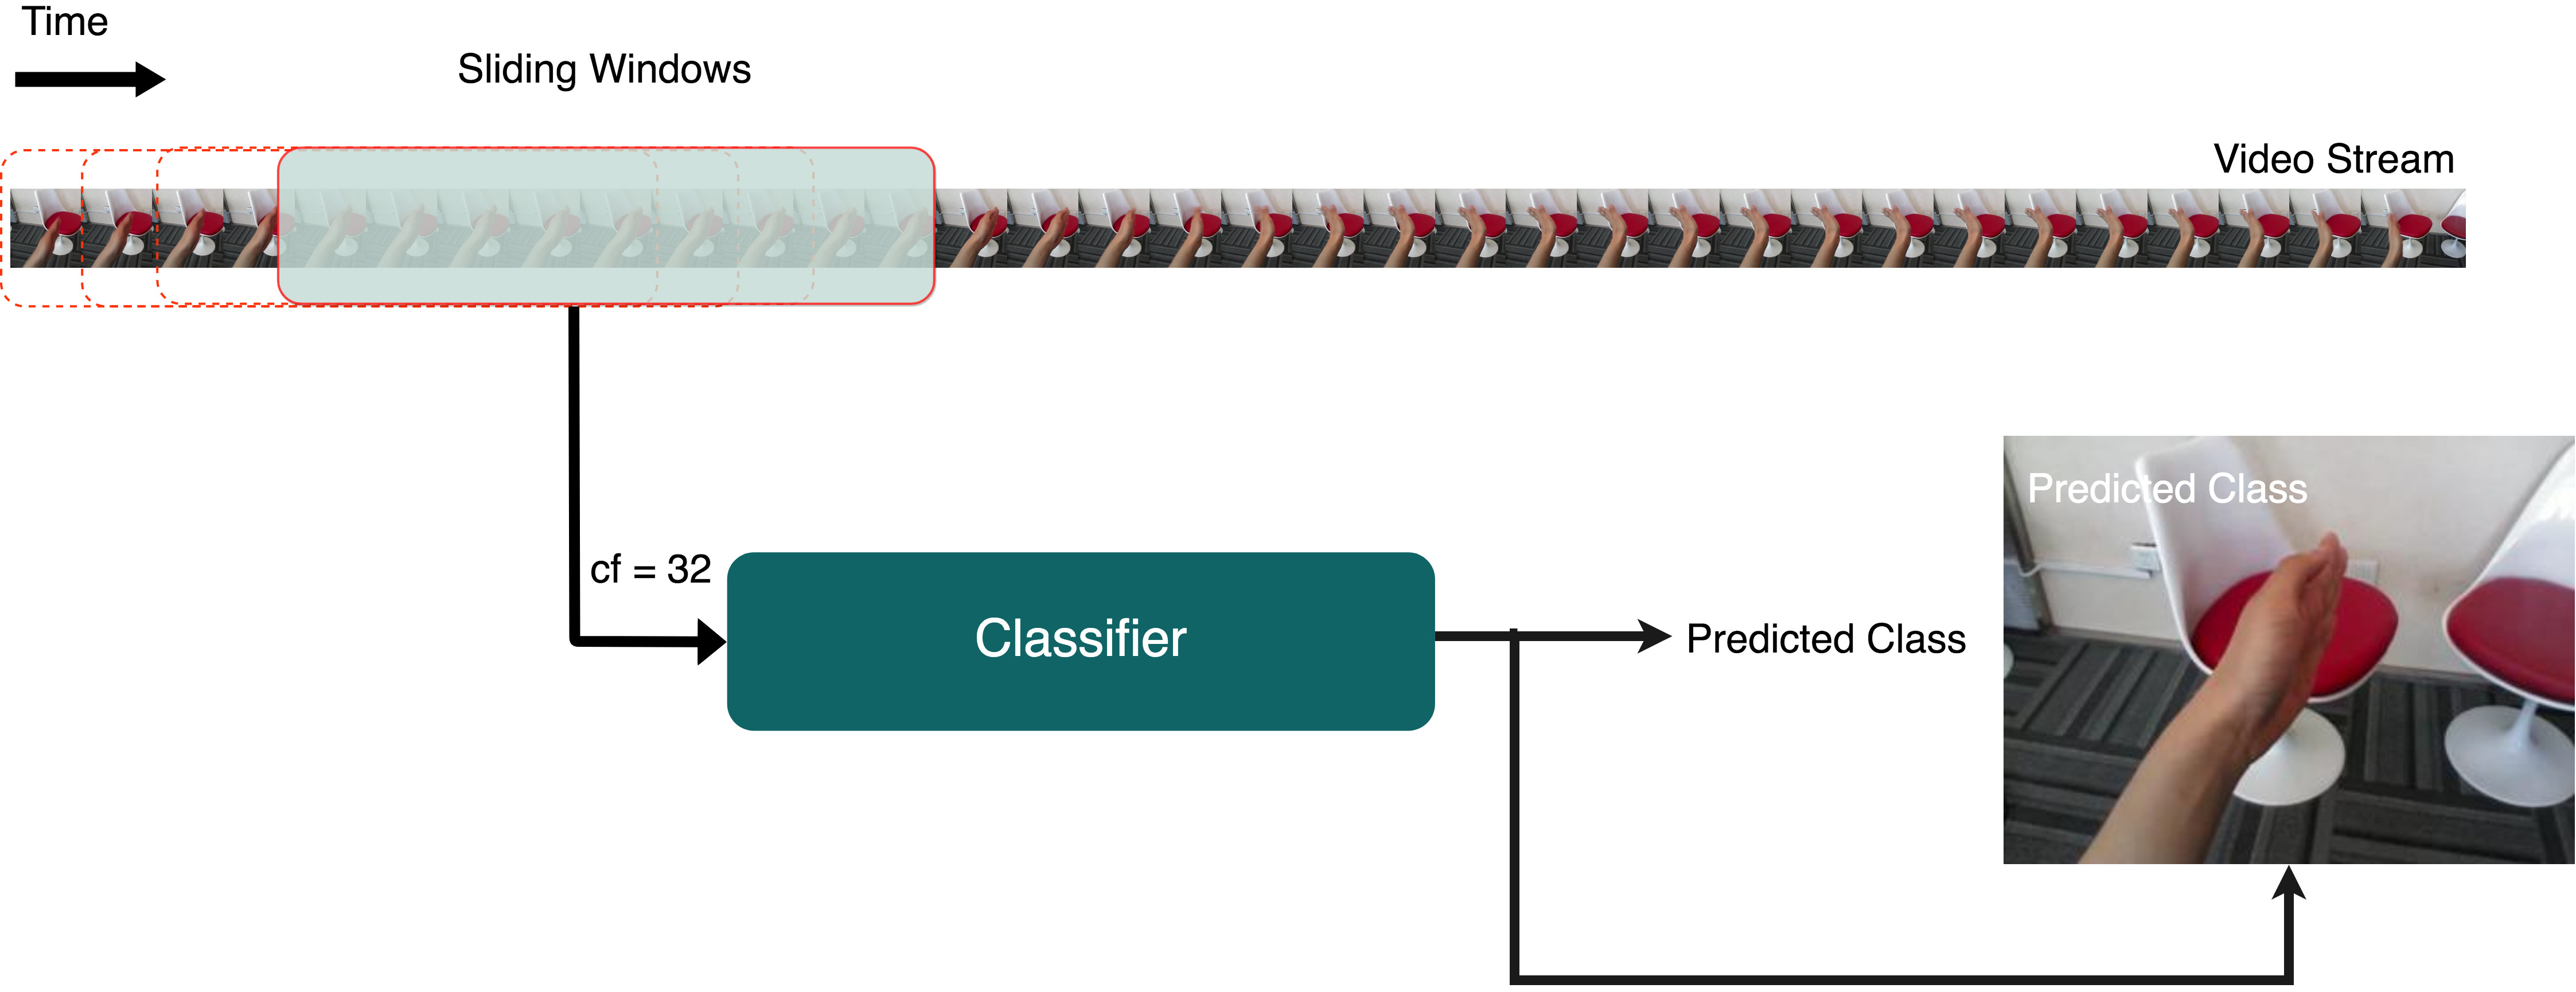
\includegraphics[width=1.0\linewidth]{figures/old_workflow}
	\caption{A basic approach of real-time gesture detection application.}
	\label{fig:old_workflow}
\end{figure}

Currently, one way of dealing with a real-time classification task could have been to run a trained model on a fixed size of a window of frames of an incoming video stream with an overlapping factor as shown in Figure \ref{fig:old_workflow}.  The overlapping strategy is essential because a gesture can start or end at the border of the window, and it is highly possible that the model would miss this.  Moreover, the timing of the detection/classification of gestures matters a lot in gesture recognition applications.   However, these models are not trained for such a scenario.  It is clear to say that frames in a window will often not be as clean as ones the model has been trained on. There could be frames that have no actions or maybe the action takes longer than it usually takes and the model will most probably miss-classify it.   Another drawback of this approach is that the model will activate more than once for the same gesture as the model go through on the same frames several times.  This brought up the following problems:
\begin{enumerate} 
\item We can never be sure when the true gesture starts since the beginning of many gestures can be very similar
\item We cannot be sure when it ends.
\item For one gesture we will have many activations.
\end{enumerate}
On the other hand,  computational resources do not need to be always used since the most of the time there is no any gesture performed in a real-time scenario.  Because of this,  we created a  two-models architecture where one light-weight model (detector) always runs and do binary classification if there is a gesture or not.   This model does not require a complicated structure most of the time since the task is more straightforward than classifying the gestures.   So if this model activates,  then the classifier will start processing. The second model (classifier) is a much more complex model than the detector because most of the resources will not be used if there is no gesture in the video stream.  After that, the classifier’s softmax outputs are post-processed to predict the outcome.  The whole structure is shown in Figure \ref{fig:workflow} (see Section \ref{sec:architecture}).\\

For the sake of eliminating these three problems above,  we propose a system has two models (detector and classifier), and a single-time activation strategy.   Figure  \ref{fig:probs} presents how decision mechanism has been done in the proposed system.\\

In the rest of this chapter,  datasets used in experiments are introduced, and then proposed network architecture is elaborated.\\
\clearpage
\section{Datasets}
\label{sec:datasets}
Vision-based human action and activity recognition tasks have an increasing trend among the computer vision community together with some applications like visual surveillance, video retrieval, and human-computer interaction.  In recent years,  more and more datasets are dedicated to human action/gesture recognition, and the use of these data sets allows us to compare different recognition systems performances.    Before the release of the  Kinetics  Human  Action  Video Dataset provided by Deepmind, research has mainly focused on learning and recognizing actions from two-dimensional (2D) approaches on frames \cite{vishwakarma_survey_2012,lim_fuzzy_2015,wang_recent_2003,guo_survey_2014}.  As a result of this,  there have been many publicly available  2D video datasets dedicated to action recognition. Review papers categorizing and summarizing their characteristics are available to help researchers in evaluating their algorithms  \cite{hassner_critical_2013,chaquet_survey_2013,ruffieux_survey_2014}.   The introduction of low-cost integrated depth sensors that can capture both RGB  (red,  green and blue) video and depth (D) information has significantly advanced the research of vision-based action recognition.   Since the first work reported in 2010 \cite{li_action_2010}, many benchmark datasets have been created to facilitate the development and evaluation of new algorithms based on 3D analysis on a stack of adjacent video frames, which is more reasonable for classification of time-related tasks such as action recognition.  On the other hand,  3D CNNs are proven to be more data-hungry in order to be trained.\\

Even though there are many vision-based datasets  available, not all of these datasets are suitable for our purpose since most of them are only providing the clips in which an action/gesture performed, which is not appropriate for training a real-time model that requires a continuous stream has regions with no action. Additionally, our research question requires a dataset to have the following attributes:
\begin{itemize}
\item To be \textbf{large enough} to train  a complex Deep Neural Network
\item Needs to be \textbf{challenging} concerning the number of gestures
\item Availability  of \textbf{no gesture part} in the videos to do continuous  classification
\item Allow us to \textbf{benchmark} our strategy and models.
\item Ability to \textbf{generalize} our approach
\end{itemize}

As a result of these prerequisites,  we evaluated proposed architecture on two dynamic hand gesture datasets:   1) EgoGesture dataset \cite{zhang_egogesture:_2018} and 2)Nvidia Dynamic Hand Gestures  Dataset  (annotated as nvGesture in this report)  \cite{nvidia_online_nodate}. \\

\subsection{EgoGesture Dataset}
\label{subsec:egogesture}
The dataset consists of videos from 50 subjects.  In total,  there are 2,081 RGB-D videos with 83 distinct dynamic or static gesture classes as shown in Figure  \ref{fig:egogesturesall}\cite{cao_egocentric_2017,zhang_egogesture:_2018}\footnote{\url{http://www.nlpr.ia.ac.cn/iva/yfzhang/datasets/egogesture.html}}.  On average each gesture class has 291 samples.\\
\begin{figure}[H]
	\centering
	\includegraphics[width=1\linewidth]{figures/Gestures_all}
	\caption{Eighty-three dynamic or static hand gesture classes in EgoGesture dataset.}
	\label{fig:egogesturesall}
\end{figure}

\begin{figure}[h]
	\centering
	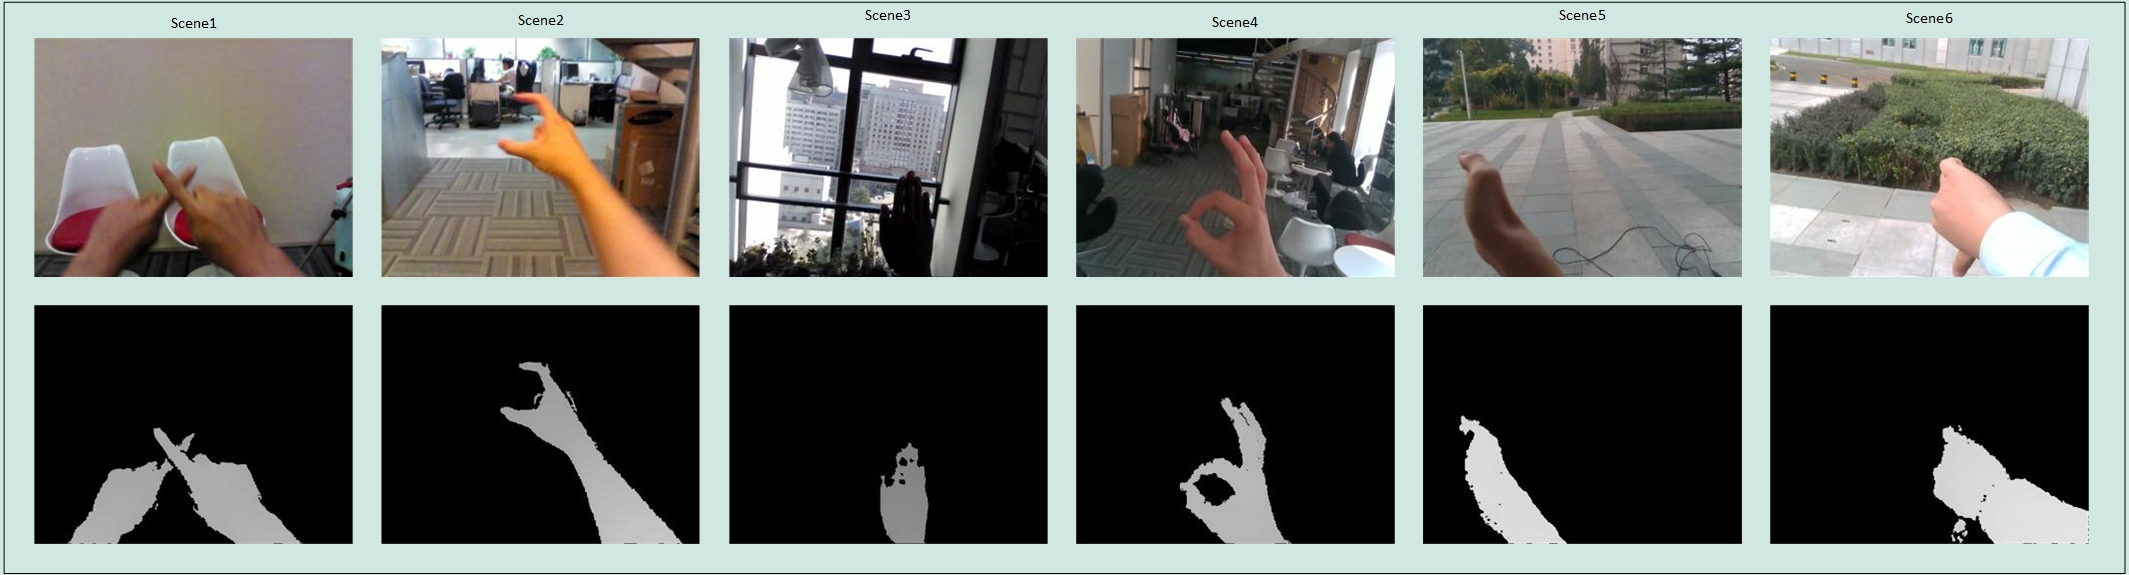
\includegraphics[width=1\linewidth]{figures/Scenes}
	\caption{Some gesture samples in 6 distinct scenes with different background and setting. Top and bottom samples are from RGB and Depth sensors, respectively} 
	\label{fig:scenes}
\end{figure}
The data is recorded in 6 different scenes while some of them are not stationary.  In \cite{zhang_egogesture:_2018,cao_egocentric_2017} each scene is described  as follows:
\begin{itemize}
\item the subject in a stationary state with a static clutter background
\item the subject in a stationary state with a dynamic background
\item the subject in a stationary state facing a window with drastic-changing sunlight
\item the subject in a walking state
\end{itemize}
and two outdoor scenes:
\begin{itemize}
\item the subject in a stationary state with a dynamic background
\item the subject in a walking state with a dynamic background.
\end{itemize}
The examples from the 6 scenes are illustrated in Figure \ref{fig:scenes}. 

Distribution of samples in each scene is illustrated in Figure \ref{fig:egogesturedist}. On the y-axis, the number of samples is shown for the corresponding subject, and each color represents the scene.  In total, we have 50 subjects (IDs from 1 to 50). Except for subjects with ID 3, 7, and 23, all other subjects recorded videos in all six scenes. It is clear that the distribution of scenes is quite balanced and on average each subject recorded about  500 samples.  This is quite important because it is harder to model to find patterns among scene, user and gestures.\\
\begin{figure}[h]
	\centering
	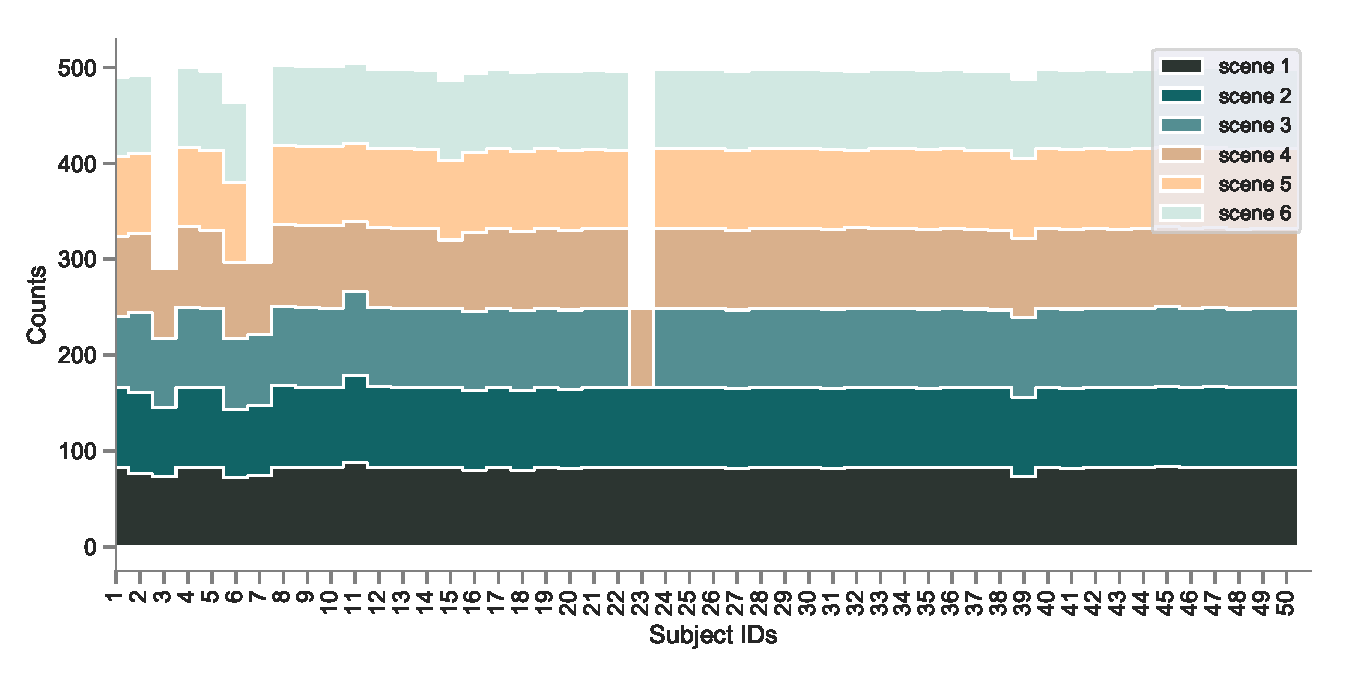
\includegraphics[width=1\linewidth]{figures/egogesturedist}
	\caption{The distribution of the gesture samples on each subject in EgoGesture dataset. The horizontal axis and the vertical axis indicate the subject ID and the sample numbers respectively.}
	\label{fig:egogesturedist}
\end{figure}

In the data collection process, Intel RealSense SR300 camera is used.  The camera is positioned on the head of each subject using a strap belt since one goal of this dataset is to capture the egocentric view of gestures.  The camera records 30 frames per second RGB-D modality videos with $640\times480$. Later in our experiments, we rescaled these images into $112\times112$. Each video consists of continuously performed gesture.  Thus, we are able to perform real-time classification experiments in continuous stream efficiently.  Besides, each clip has the gesture part of video  is labeled by providing start and end index of frames.  This allows us to train our offline models. \\

\begin{figure}[H]
	\centering
	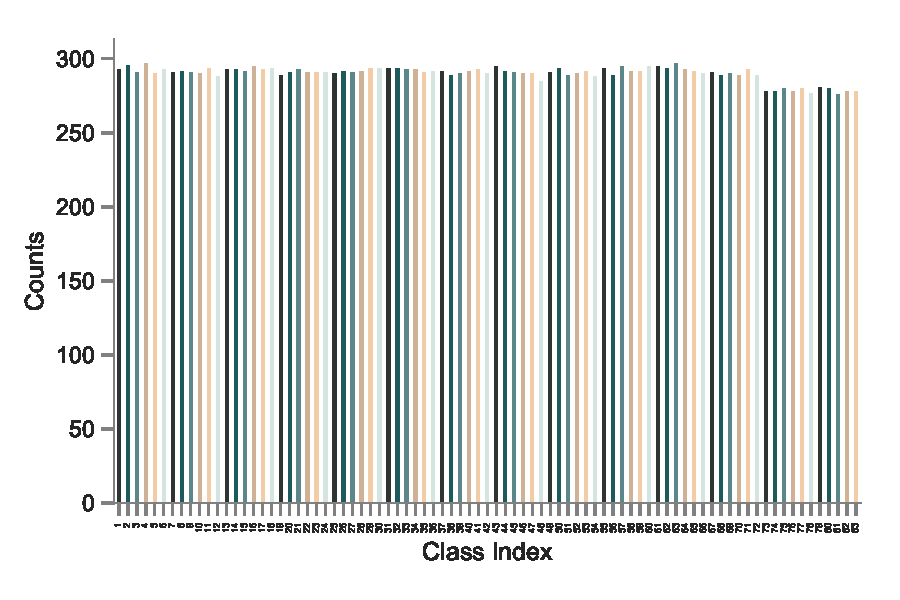
\includegraphics[width=0.8\linewidth]{figures/egogestureclassdist}
	\caption{Sample distributions per gesture class in the EgoGesture dataset.}
	\label{fig:egogestureclassdist}
\end{figure}

Figure \ref{fig:egogesturedist} shows the distribution of data over 6 scenes, and it is clear to say that it is quite balanced.  This is important for our training and evaluation phase.  Trained model can learn the structure of a scene more than the others, and this will mislead the model if the distribution is not balanced over the scenes.  On the other hand,  in Machine Learning (ML) task, the distribution of the classes/gestures plays an important role\cite{wei_role_2013}.  If dataset unbalanced and samples for some classes is more than samples from others in an exaggerated scenario, then the model will most probably only learn this class and always predict this class regardless of the input.   This is because,  in training, most of the loss will come from misclassification of those samples from majority classes, and model will be able to decrease the loss by correctly classifying only these samples but not others.   In the EgoGesture dataset, The classes are quite balanced as it is shown in Figure \ref{fig:egogestureclassdist}, And on average there are 291 gesture samples per classes.\\
\begin{figure}[h]%
\centering
\subfigure[]{%
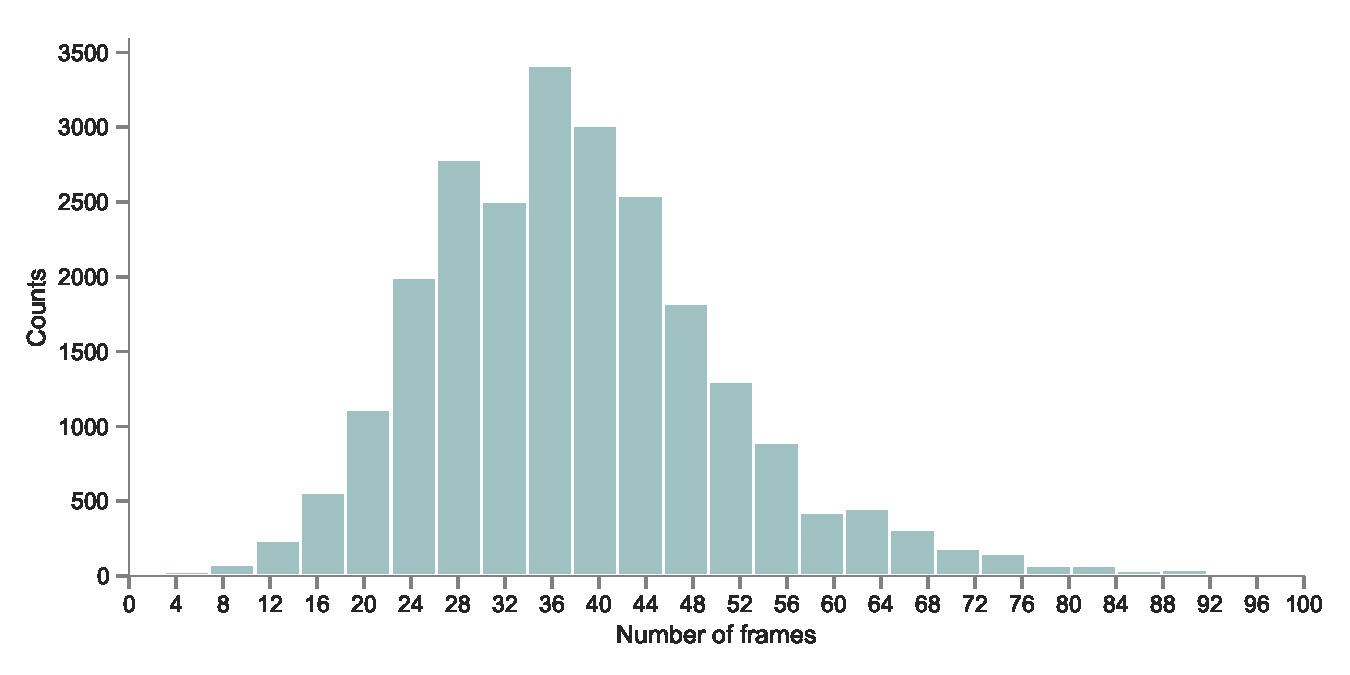
\includegraphics[height=0.25\linewidth]{figures/egogestureframesdist.pdf}}%
\label{fig:framedist1}%
\qquad
\subfigure[]{%
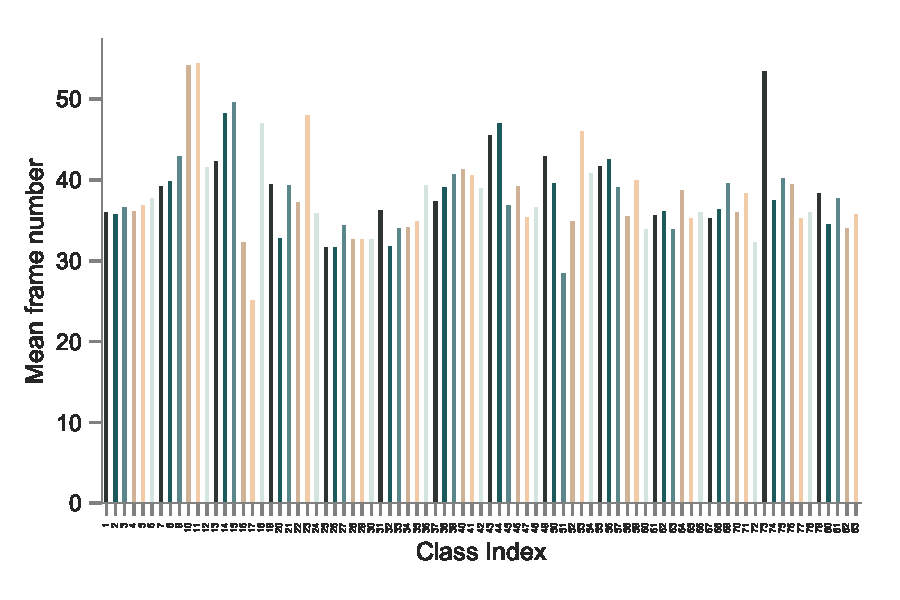
\includegraphics[height=0.25\linewidth]{figures/egogestureframedistperclass}}%
\caption{(a) Distribution of the number of frames per gesture. 
(b) Distribution of the number of frames for each gesture class in the EgoGesture dataset. }
\label{fig:egogestureframeall}
\end{figure}

In vision-based gesture recognition tasks, the number of frames per gesture plays a vital role in the decision of hyperparameters for 3D kernels.  In Figure  \ref{fig:egogestureframeall} (a),  it is shown that the number of frames per gesture across EgoGesture dataset has a Gaussian-like distribution whose mean is 38.4. The min and max number of frames are 3 and 196 respectively.  In this figure, however, we used samples in range 0-100, in which 99\% of the data lies, for the sake of better view of the distribution. There are only 37 samples which have less than eight frames and 79 samples with more than  100 frames. We realized that gesture with id 17, which is ”sweep diagonal” is mostly performed less than eight frames.  So  the mean number of frames across gestures is investigated, see Figure \ref{fig:egogestureframeall} (b). There is no any gesture stands out drastically from others.   Thus,  it is safe to assume the number of frames per gesture is not so much dependent on gesture class. \\

\subsection{NVIDIA Dynamic Hand Gestures Dataset}
\label{subsec:nvidia}
\begin{figure}[H]
	\centering
	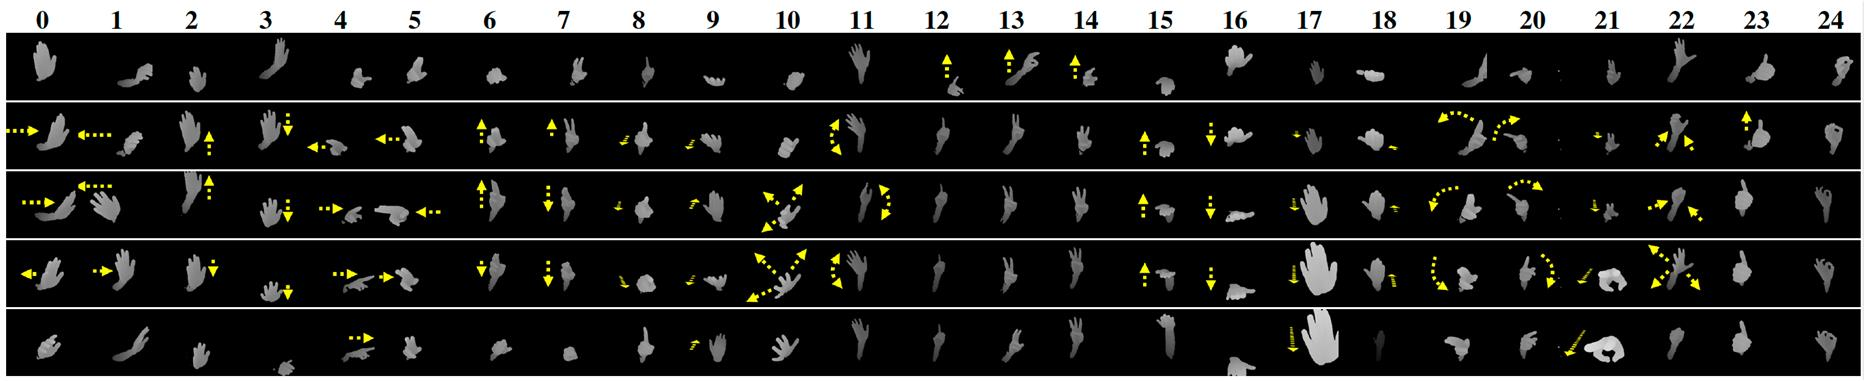
\includegraphics[width=1\linewidth]{figures/nvidia_classes_all}
	\caption{NVIDIA Dynamic Hand Gesture Dataset (nvGesture) classes. In total , there are twenty-five dynamic hand gestures (0-24) and each column represents each one of them. In bottom rows, yellow arrows illustrate the movement of hands. (This figure is from Molchanov et al. \cite{molchanov_online_2016} and more detailed information can be found there)}
	\label{fig:nvgesturesall}
\end{figure}

In the nvGesture dataset, there are in total 1050 video recordings for training and 482 recordings for testing from 20 different subject performing in a car simulation environment with different lightening scenarios. It includes 25 distinct gestures, shown in Figure \ref{fig:nvgesturesall}, while 6 of them being static gestures. Besides, the start and end frame of each gesture clip in nvGesture are not precisely cropped while each is represented by exactly 81 frames. Each gesture class has on average 61.2 recordings as it is shown in Figure \ref{fig:nvidiaclassdist}, which is much less than the average number of samples (291) per a gesture class in the EgoGesture. Moreover, Figure \ref{fig:nvidiaclassdist} illustrates the sample distribution for each classes, and it is clear to say that the dataset has a balanced class distribution which is critical in the training. \\
\begin{figure}[h!]
	\centering
	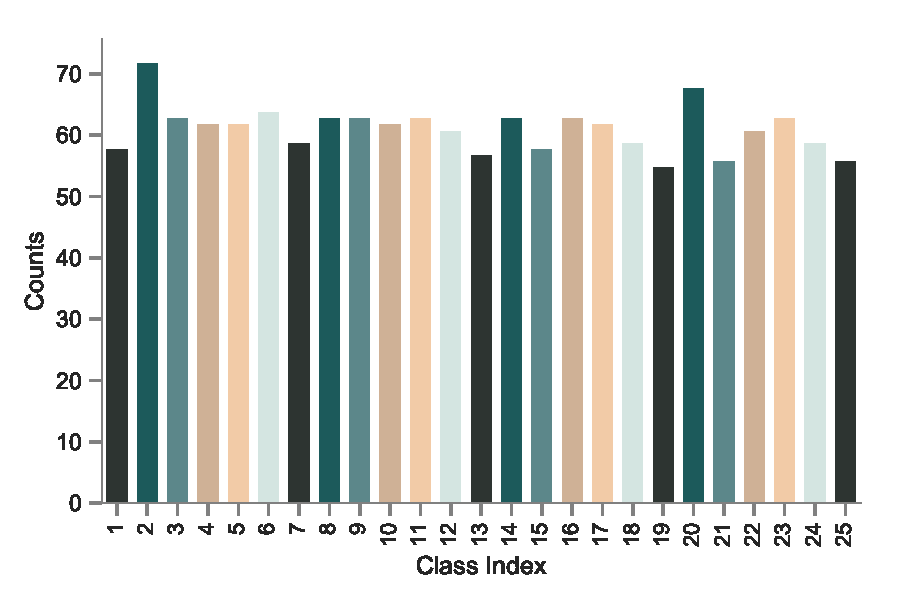
\includegraphics[width=0.5\linewidth]{figures/nvidiaclassdist}
	\caption{Sample distributions per gesture class in the nvGesture dataset.}
	\label{fig:nvidiaclassdist}
\end{figure}

In the nvGesture dataset, a SoftKinetic DS325 sensor was used to capture front view color and depth videos, and a DUO 3D camera was used to record stereo IR (left, disparity). Both cameras capture $320\times240$ pixels at 30 frames per second (fps) as it is introduced in \cite{molchanov_online_2016}. Overall, it contains optical flow and 4 other modalities: RGB, depth, IR-left, and IR-disparity. In our analysis,  we only used first view  RGB and depth modality videos  as it is more discriminative and natural view of the task. \\  

\section{Architecture}
\label{sec:architecture}
\begin{figure}[h!] 
	\centering
	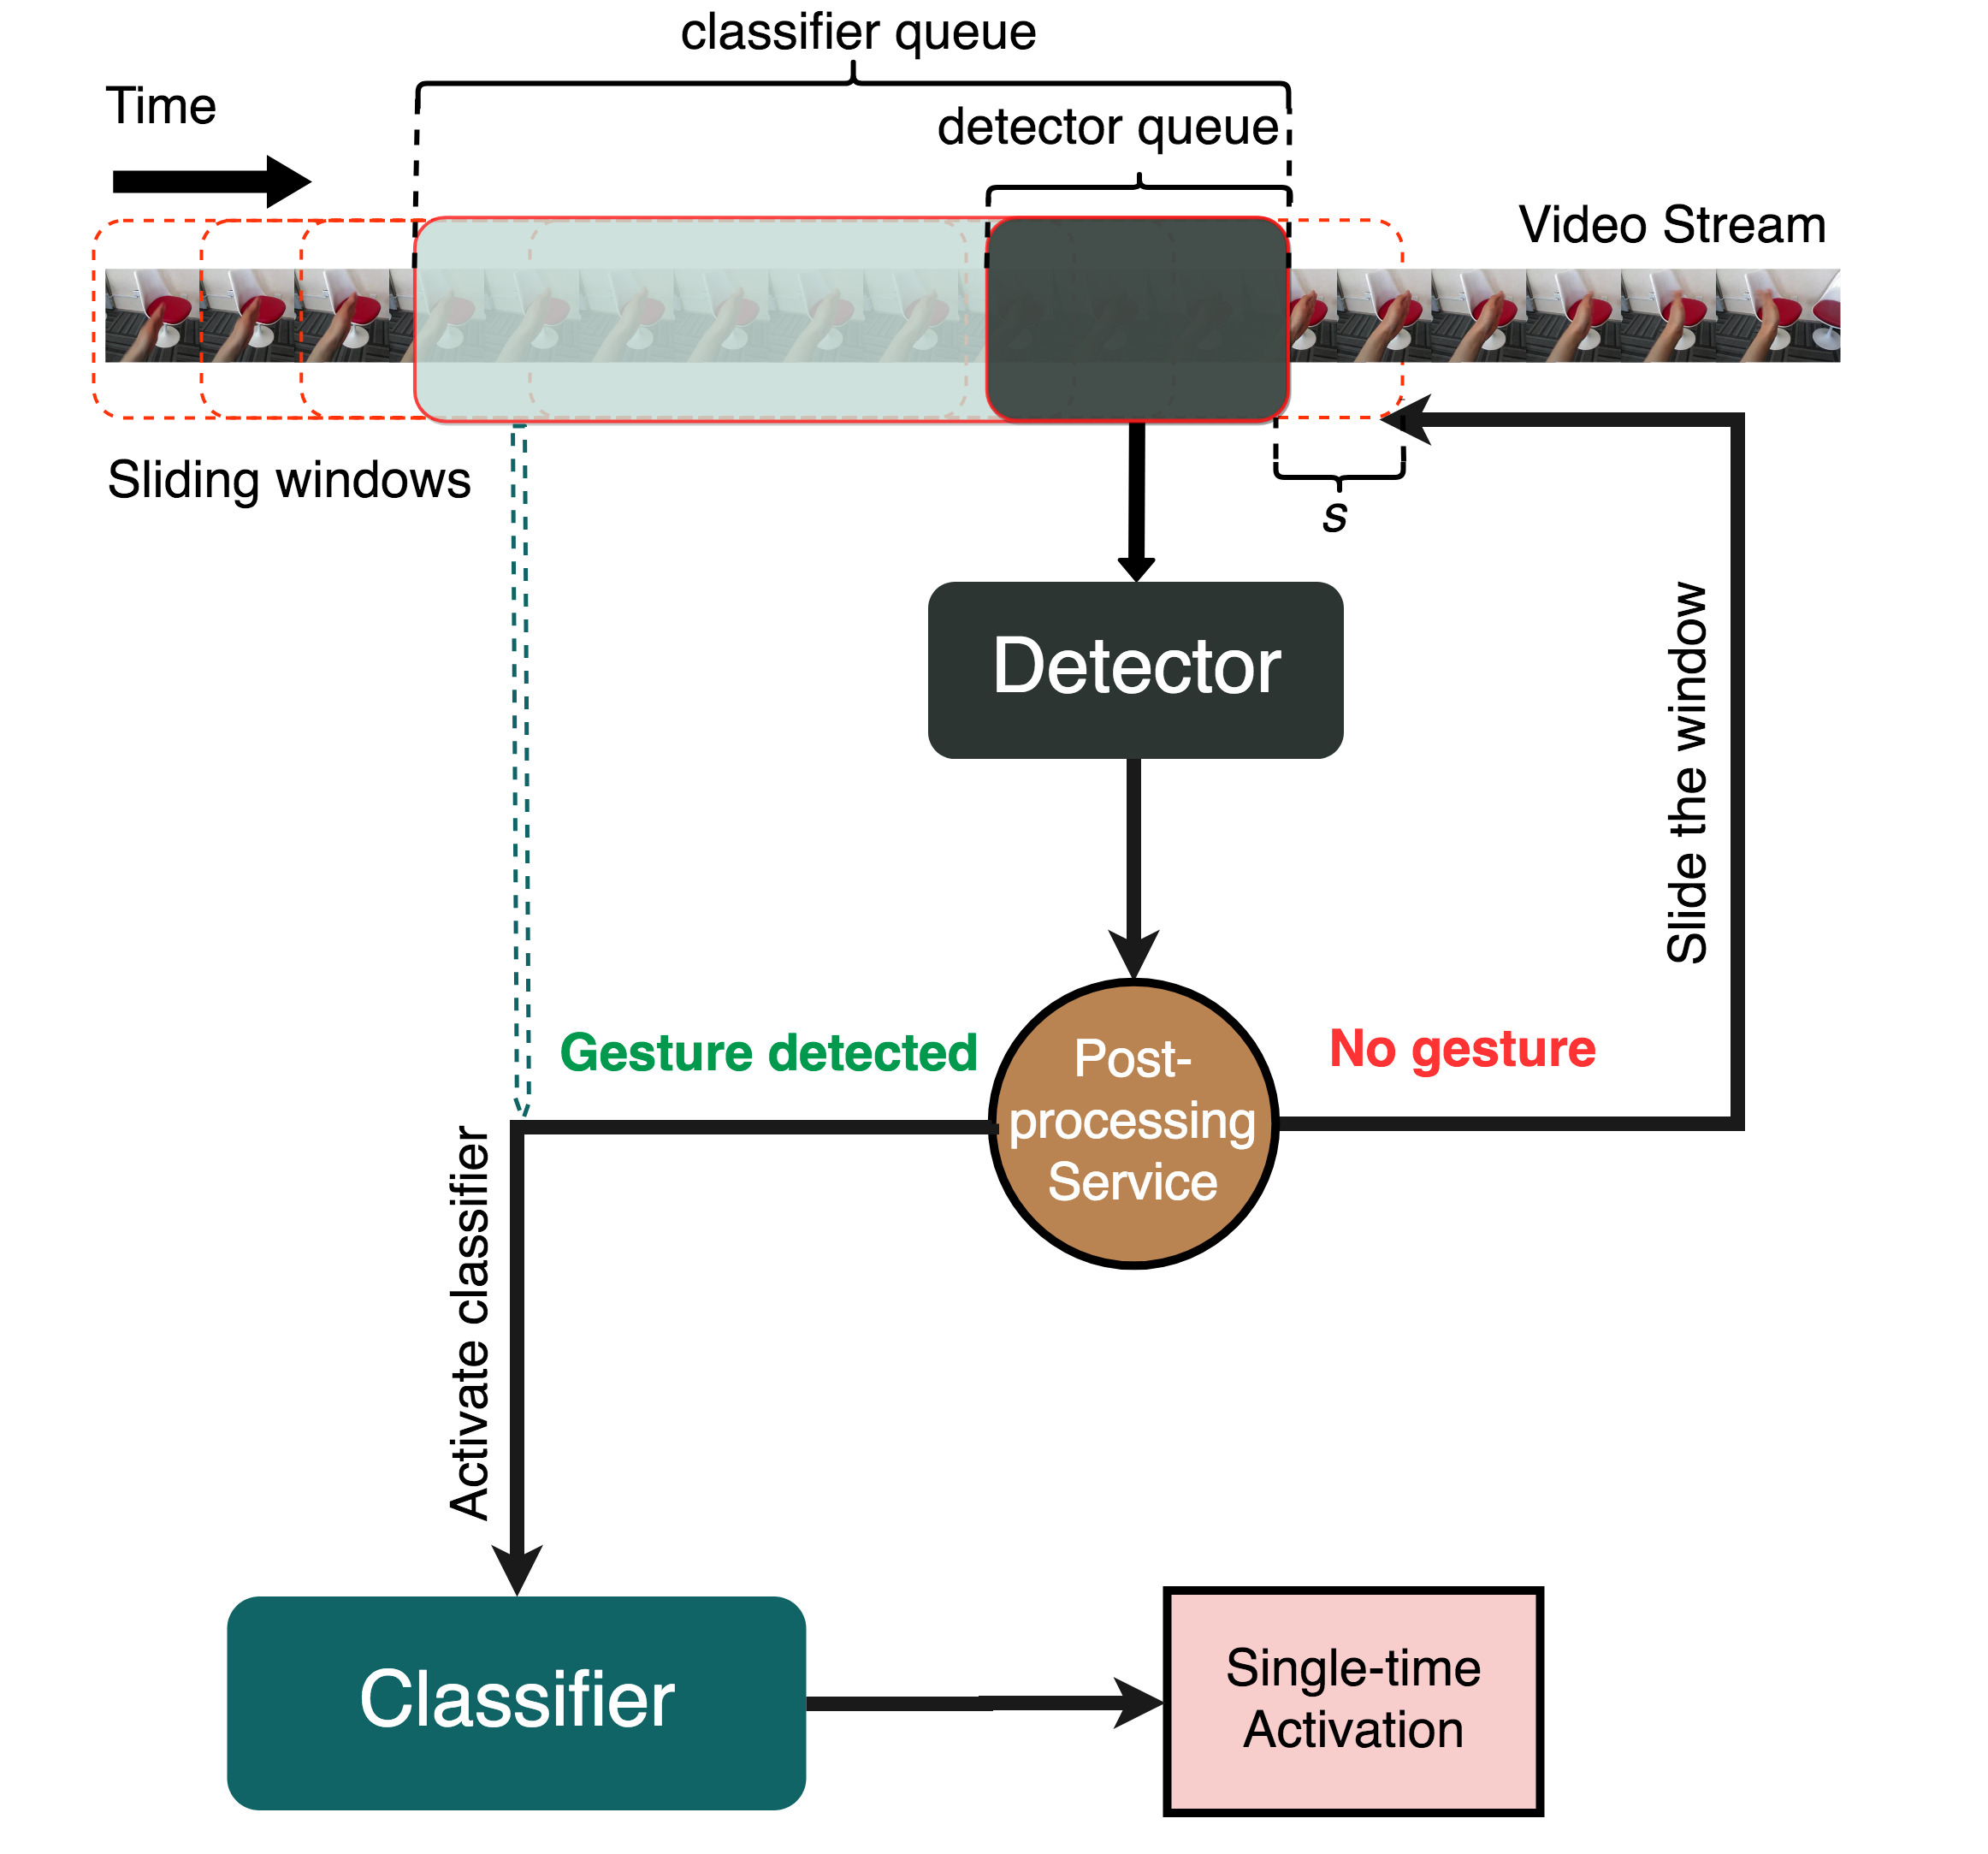
\includegraphics[width =0.9\textwidth]{figures/arch}
	\caption{The general workflow of the proposed two-model hierarchical architecture. Sliding windows with stride \textit{s} run through incoming video frames where detector queue placed at the very beginning of classifier queue. If detector recognize an action/gesture then the classifier is activated. Both detector and classifier outputs are post processed for a more robust performance, and decision is made using single-time activation block where only one activation occurs per performed gesture.}
	\label{fig:workflow}
\end{figure}

In this section, we elaborate on our two-model hierarchical architecture that integrates any state-of-the-art models into  real-time gesture recognition applications as efficiently as possible. After introducing two-model hierarchical architecture, training details are described. And finally, we give a deep understanding into the used post processing strategies that allow us to have single-time activation per gesture in real-time. \\

Recently, with the availability of large datasets, CNN based models have proven their ability in action/gesture recognition tasks. 3D CNN architectures especially stands out for video analysis since they make use of the temporal relations between frames together with their spatial content. However, there is no clear description of how to use these models in a real-time dynamic systems. With our work, we aim to fill this research gap.\\

Figure \ref{fig:workflow} shows illustrates the used workflow for an efficient real-time recognition performance using a sliding window approach. In contrary to offline testing, we do not know when a gesture starts or ends. Because of this, our workflow starts with a detector which is used as a switch to activate classifier if a gesture gets detected. Our detector and classifier models are fed by a sequence of frames with size $m$ and $n$, respectively such as $n \ll m$ with an overlapping factor as shown in Figure \ref{fig:workflow}. The stride used in the sliding window is $s$ and it is same for both the detector and the classifier. Although higher stride provides less resource usage, we have chosen $s$ as 1 since it is small enough not to miss any gestures and allows us to achieve better performance. In addition to the detector and classifier models, one post-processing and one single-time activation service is introduced to the workflow in order to achieve single-time activation per gesture. In the next parts, we are going to explain these blocks in detail.\\

As the overall accuracy of our system highly depends on the performance of the detector, we require the detector to be robust and accurate in detection of true positives, meaning that it must have high recall value.  For the sake of the former, detector runs on a smaller number of frames than classifier which we refer to as detector queue.   For the latter, detector queue is placed on the very beginning of classifier queue as shown in Figure \ref{fig:workflow}. Additionally,  we use some common filters like median,  moving average or exponentially weighted moving average in the post-processing service in order to clear out miss classifications.  This is not required for offline testing.   However, in online testing, we can make use of consecutive prediction scores of the models and allow the model to activate only once per gesture as we are using sliding windows with a stride length on the incoming video data.   We believe that this is the first work that shows how to use such post-processing techniques in vision-based gesture recognition tasks.\\
\begin{figure}[H]
	\centering 
	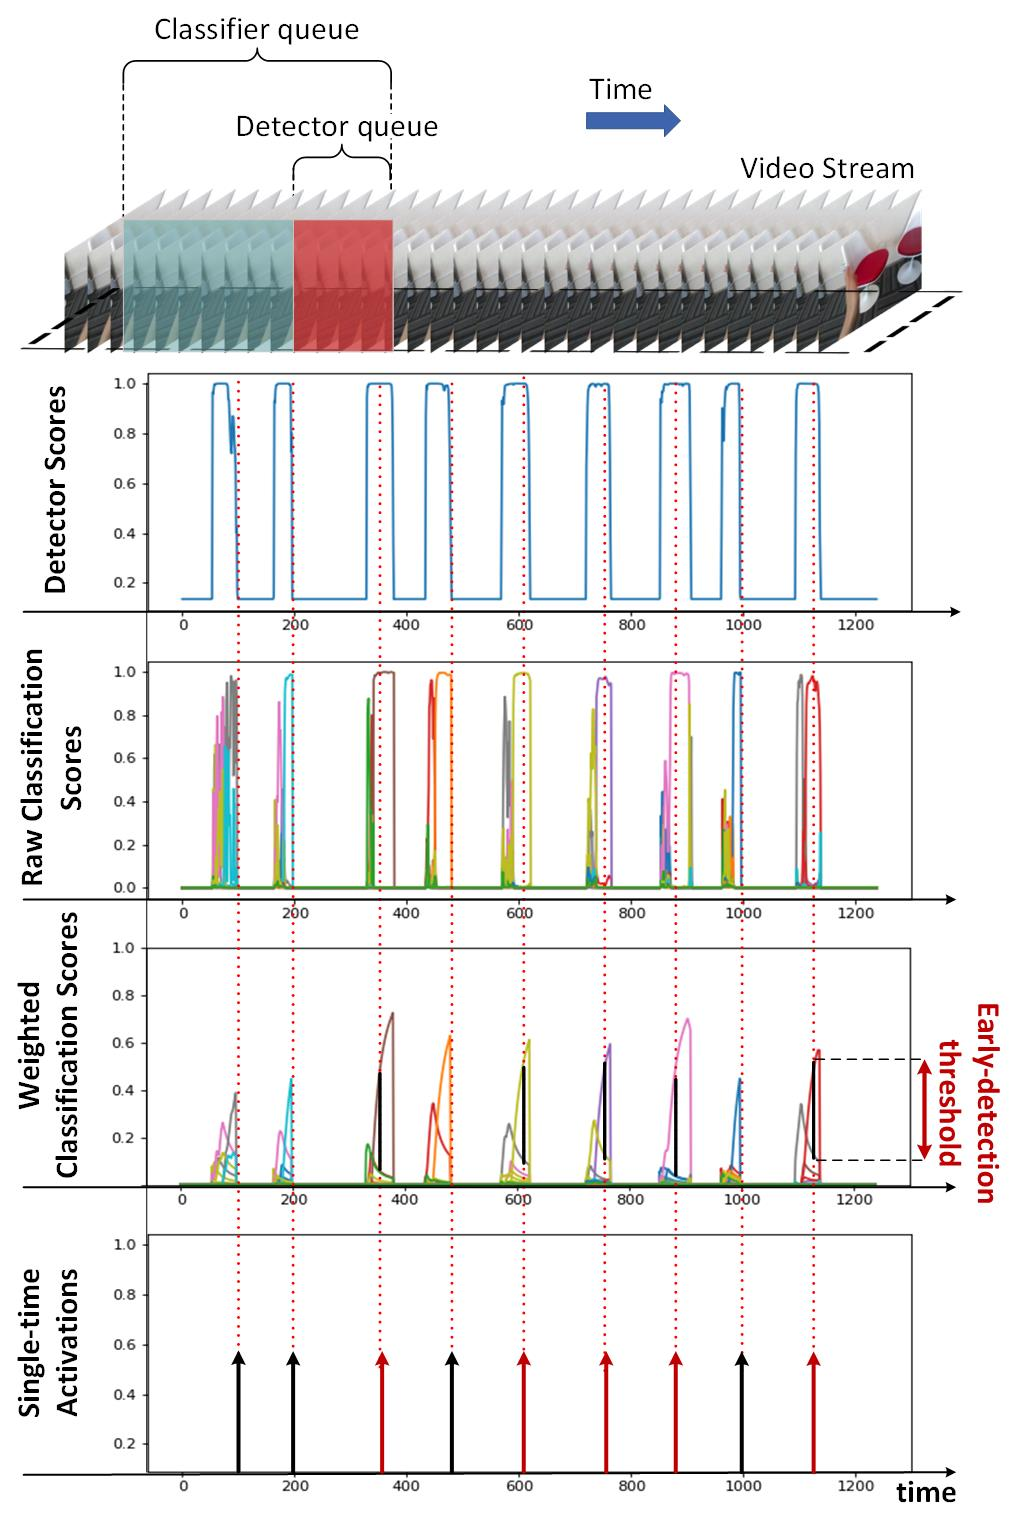
\includegraphics[width=0.8\textwidth]{figures/probs}
	\caption{Proposed pipeline illustrations for real-time gesture recognition. When we run our proposed structure over an incoming video stream by sliding one frame at each iteration, these results are achieved. First figure shows detector probability scores for class 1 (\textit{gesture}), second figure illustrates each classes classification score with different colors, third one is weighted-average of classification scores with weight function $W(x) = 1/(1+\exp^{-0.2\times(x-9)})$ where $x$ is the iteration index, and the bottom one illustrates single-time activations such that red arrow represents early detection and black one is for detection after gesture ends.}
	\label{fig:probs}
\end{figure}

Figure \ref{fig:probs} shows the transformation of the classifiers probability scores through the proposed architecture shown in Figure \ref{fig:workflow}. The difference between the weighted-average of the scores and the raw scores plots proves that the true gesture can be emphasized and detected more precisely as the true information in the gesture lies at the mid-late range of it. Additionally, the early detection strategy is shown with the help of an threshold level. Finally, the bottom image shows the activations of each gestures in real time evaluation (red colored arrows represent early detections). In total we are able to successfully detect all true classes for this sample (EgoGesture dataset, Subject 4, Scene 2 and recording 5), while 5 of them being early detected.\\
\subsection{Detector}
\label{subsec:detector}
\begin{figure}[t!]
	\centering
	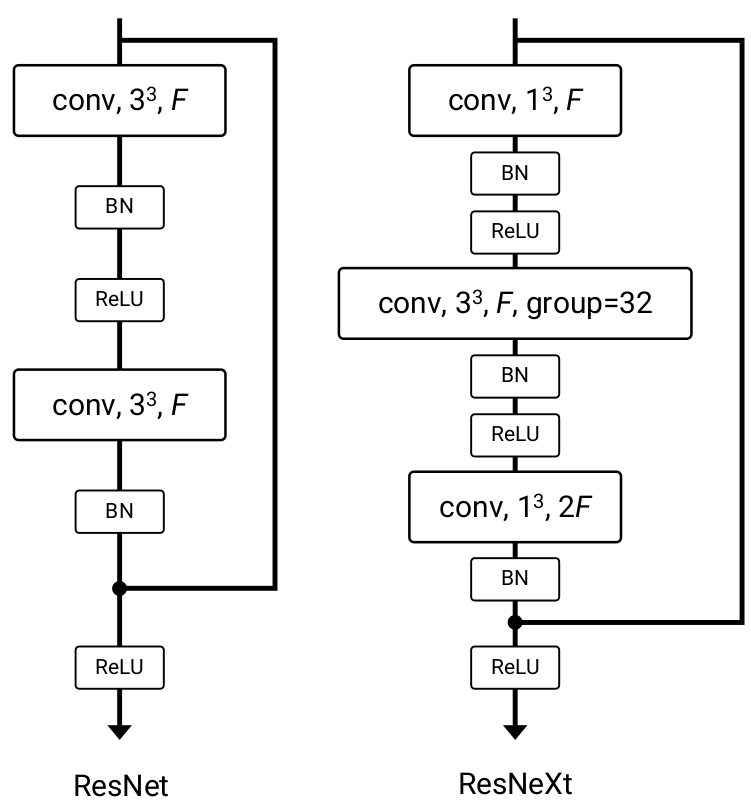
\includegraphics[width=0.5\textwidth]{figures/blocks}
	\caption{ResNet and ResNeXt blocks used in the detector and classifier architectures.}
	\label{fig:blocks}
\end{figure}
Detector runs on the images in the detector queue in every iteration, and the purpose of this model is to detect if any action is performed,  ”1” for \textit{gesture} and ”0” for \textit{no gesture}.  Its main and only role is to act as a switch for the classifier model, meaning that if the detector predicts ”1” classifier is activated and fed by frames in its own window. However, it is possible that for some frames there is no hand present and it can predict \textit{no gesture} while a gesture being performed.  In order to decrease this possibility, we post-process the output probabilities, and after that, we set a threshold $d_{th}$ for the consecutive number of \textit{no gesture} predictions to deactivate classifier.\\

The purpose of the detector is to distinguish between \textit{gesture} and \textit{no gesture} classes by running on a sequence of images that detector queue masks at every iteration. Its main and only role is to act as a switch for the classifier model, meaning that if it detects a \textit{gesture}, then classifier is activated and fed by the frames in classifier queue.\\

As the overall accuracy of this system highly depends on the performance of detector, we require the detector to be (i) robust and (ii) accurate in detection of true positives, meaning that it must have high recall value. For the sake of the former, detector runs on smaller number of frames than classifier which we refer as detector and classifier queues. For the latter, detector queue is placed on the very beginning of classifier queue as shown in Figure \ref{fig:workflow}, and this enable the detector to activate the classifier whenever a gesture starts regardless of the gesture duration.\\ 
\begin{table}[t!]
	\centering
	\begin{tabular}{c|c|c|c}
	\hline
	\textbf{Layer}    & \textbf{Output Size}   & \textbf{ResNeXt-101}  & \textbf{ResNet-10} \\ \hline
	conv1    & L x 56 x 56   & \multicolumn{2}{c}{3x7x7, stride (1, 2, 2)}                                                                 \\ \hline
	conv2\_x & L x 56 x 56   & N:3, F:128                                            & N:1, F:16                                            \\ \hline
	conv3\_x & L/2 x 56 x 56 & N:24, F:256                                           & N:1, F:32                                            \\ \hline
	conv4\_x & L/4 x 56 x 56 & N:36, F:512                                           & N:1, F:64                                            \\ \hline
	conv5\_x & L/8 x 56 x 56 & N:3, F:1024                                           & N:1, F:128                                           \\ \hline
         & 1 x 1 x 1     & \multicolumn{2}{c}{\begin{tabular}[c]{@{}c@{}}global average pooling,\\ fc layer with softmax\end{tabular}} \\ \hline
	\end{tabular}
    \caption{Detector (ResNet-10) and Classifier (ResNeXt-101) architectures. F corresponds to the number of feature channels in the blocks shown in Figure \ref{fig:blocks}, N is the number of blocks in corresponding layer, and L is the number of frames fed to the model.}
	\label{tab:architecture}
\end{table}

%Additionally, we used some common filters (moving median, moving average and exponentially-weighted moving average) in the post processing service in order to clear out miss classifications in online testing. This filtering strategy allowed us to make use of consecutive prediction scores of the models. We believe that this is the first work that shows how to use such post-processing techniques in vision-based gesture recognition tasks.

The proposed detector architecture is build upon two critical assumptions: \textit{(1)} The detector should be a lightweight model since it is running continuously, and \textit{(2)} the detector should not miss any \textit{gesture} classes. For the sake of \textit{(1)}, we focused on a relatively shallow 3D CNN architecture, and decided to use ResNet-10 with reduced number of features in each layer. ResNet-10 architecture is given in Table \ref{tab:architecture} which uses the ResNet block given in Figure \ref{fig:blocks}. In order to achive \textit{(2)}, the detector model is trained with a weighted-cross entropy loss in order to decrease the likelihood of false positives. Class weights for class \textit{no gesture} and \textit{gesture} is selected as 1:3, respectively as our experiments showed that this proportion is sufficient to have 98+\% and 97+\% recalls in in EgoGesture and nvGesture datasets, respectively. Besides that, we post-process the output probabilities, and set a counter for the consecutive number of \textit{no gesture} predictions in decision of deactivating classifier. As an input to our detector,We have analyzed the input modalities of RGB, Depth and the data level fusion of both of them (RGB-D) \cite{kopuklu2018motion}. \\
\subsection{Classifier}
\label{subsec:classifier}
In computer vision (CV) area, gesture recognition has been one of the main tasks, and researchers have come quite a way since the beginning of the CV area. Most of these researches are about achieving the highest accuracy on some selected benchmark datasets.  Rarely,  the focus is on how to use these models in a real-time scenario.  In this work, we aim to integrate these developed models which have reasonable accuracy rate into a real-time application.\\

Since we do not have any limitation regarding the size or complexity of the model, any architecture with good performance in this task can be selected for classification.  This lead us to use two recent 3D CNN architectures (C3D \cite{tran_learning_2014}, and ResNext-101 \cite{he_deep_2015}) as our classifier model.  However, it is important to note that our architecture is independent of the model type.\\

Since the invention of \textbf{LeNet-5} \cite{lecun_gradient-based_1998} in LeCun et al.  which is considered as the first Convolutional neural network (CNNs) architecture, CNNs has found its position as the most successful method to learn, recognize patterns from images.  In this section, we first introduce the underlying architecture of C3D and one of its variant (called ResNext-101 \cite{xie_aggregated_2016}) that we used as a classifier in this work because we mainly focused on these two methods in this thesis and then explain our training strategies for the classifier.\\

For C3D model, we have used the exact same model as in \cite{tran_learning_2014} but the last two fully connected layers where we have used 2048 nodes instead of 4096. For ResNeXt-101, we have followed the guidelines of \cite{hara3dcnns} and chose the model parameters as given is Table \ref{tab:architecture} with ResNeXt blocks as in Figure \ref{fig:blocks}. The most basic ResNet block has two convolutional layers followed by a ReLU activation, and there is a connection between input and output after which there is another  ReLU operation.   This structure is first introduced in \cite{he_deep_2015}, and it allows for training more than  100 layers.   This revolutionized Computer  Vision/ Deep Learning community as training deep networks without overfitting is one of the main challenges.  In \cite{he_identity_2016}, researchers achieved to train even 1001-layered ResNet.  Because of its appealing results in many tasks,  ResNet quickly became popular in the research community. There are many variants of ResNet developed in 3 years by changing the structure of the residual block. One of the most successful ones is called ResNext.\\

As the number of parameters for 3D CNNs are much more than 2D CNNs, they require more training data in order to prevent overfitting. Because of this reason, we pretrained our classifier structures first on Jester dataset \cite{twentybn_20bn-jester_nodate}, which is the largest publicly available hand gesture dataset, and then fine tune our model by using this pretrained model as initialized.  This approach increased the accuracy and shortened the training duration drastically. \\

\textit{Training Details: } We used stochastic gradient descent (SGD) with Nesterov momentum = 0.9, damping factor = 0.9, and weight decay = 0.001 as optimizer. After pretraining on Jester dataset, the learning rate is started as 0.01, and divided by 10 at $10^{th}$ and $25^{th}$ epoches.\\

For regularization, we used a weight decay ($\gamma = 1 \times 10^{-3}$) is applied on all the parameters of the network. We also used dropout layers in C3D and several data augmentation techniques through out training.\\

In case of augmentation methods, three methods were used: (1) Each image is randomly cropped with size $112 \times 112$ at corners such that one of 4 corners is selected uniformly. (2) Spatial elastic displacement with $\alpha = 1$ and $\sigma = 2$ is applied after cropping images. For temporal augmentation , on the other hand, (3) we randomly select consecutive frames with input sample duration from the entire gesture videos. If the sample duration is more than number of frames in target class, we append frames starting from very first frame in a cyclic fashion. We also normalized the images into 0-1 scale using mean and standard deviation of the whole training sets in order to force models to learn faster.\\

During offline and online testing, we scaled images into $112 \times 112$ and then only normalization is performed for the sake of consistency between training and testing. The same training details are used for detector and classifier models.\\
\clearpage
\subsection{Post-processing}
\label{subsec:pp}
\begin{figure}[b!]
	\centering
	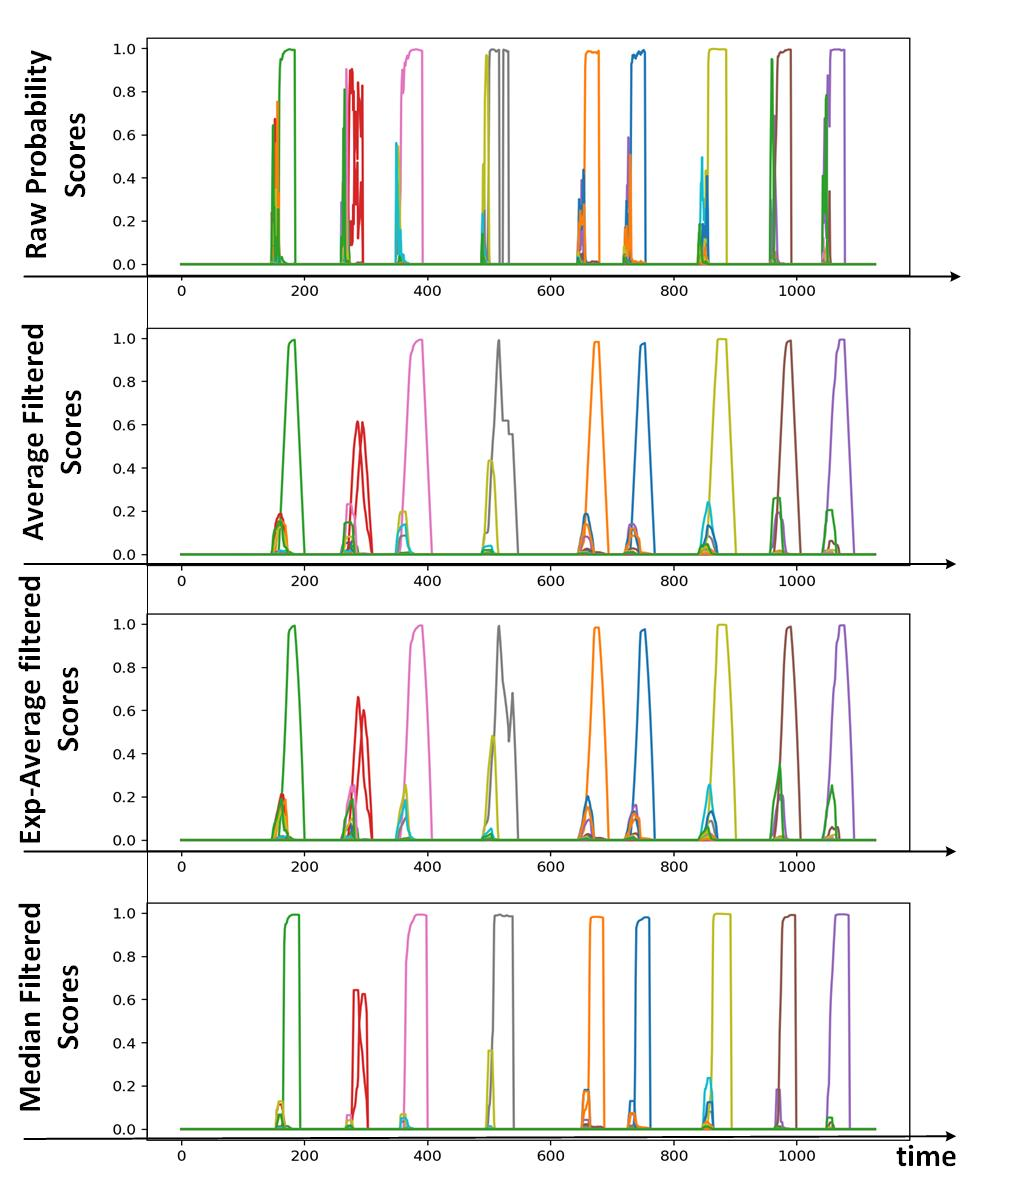
\includegraphics[width=0.8\textwidth]{figures/post}
	\caption{An illustration of the effect of post-processing filters on classification scores of each class: raw, uniformly-averaged, weighted-averaged and median filtered probability scores from top to bottom.}
	\label{fig:post}
\end{figure}

In dynamic hand gestures, it is possible that the hand gets out of the camera view  while performing gesture. Even though previous predictions of the detector are correct, any misclassifications reduce the overall performance of the proposed architecture. In order to make use of previous predictions, we add the raw softmax probabilities of the previous detector predictions into a queue ($q_k$) having a size of $k$, and apply filtering on these raw values resulting in final detector decisions. With this approach, detector increases its confidence in decision making, and clears out most of the misclassifications in consecutive predictions. The size of the queue ($k$) is selected as 4, which achieved the best results for stride $s$ of 1 in our experiments. \\

We have applied $(i)$ average, $(ii)$ exponentially-weighted average and $(iii)$ median filtering separately on the values in $q_k$. While average filtering simply takes the mean value of the $q_k$, median filtering takes median. Exponentially-weighted average filtering, on the other hand, uses weighting function of  $w_i = \exp^{-{{(1-(k-i))}/k}}$ where $i$ stands for the index of $i^{th}$ previous sample and satisfies $0 \leq i < k$, and $w_i$ is the weight for the $i^{th}$ previous sample. For better understanding, we tested different filtering approaches on the multi-classification task, shown in Figure \ref{fig:post}. \\



%These methods cancels out most of the miss classifications. We observed that median filter forces the true class stands out even more and clears of misclassifications due to the camera view. As a result, we used median filtered scores with queue size $k = 2$ in our architecture. In \cite{molchanov2016online}, a similar results are achieved by training the model with CTC loss; however, in Figure SOMETHING!!!!!, it is shown that we can force the true gestures stands out even more with much less effort.

\begin{figure}[b!]%
\centering
\subfigure[]{%
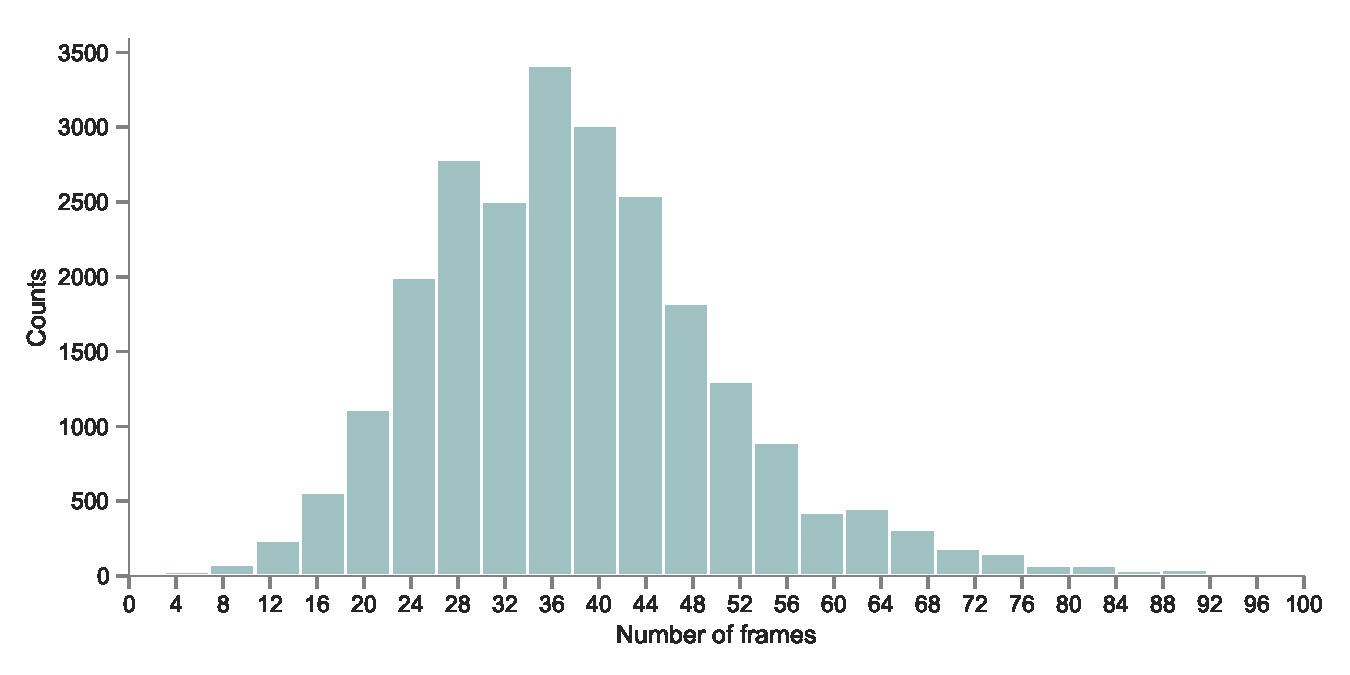
\includegraphics[width=0.45\linewidth]{figures/egogestureframesdist}}%
\label{fig:egoframe}%
\qquad
\subfigure[]{%
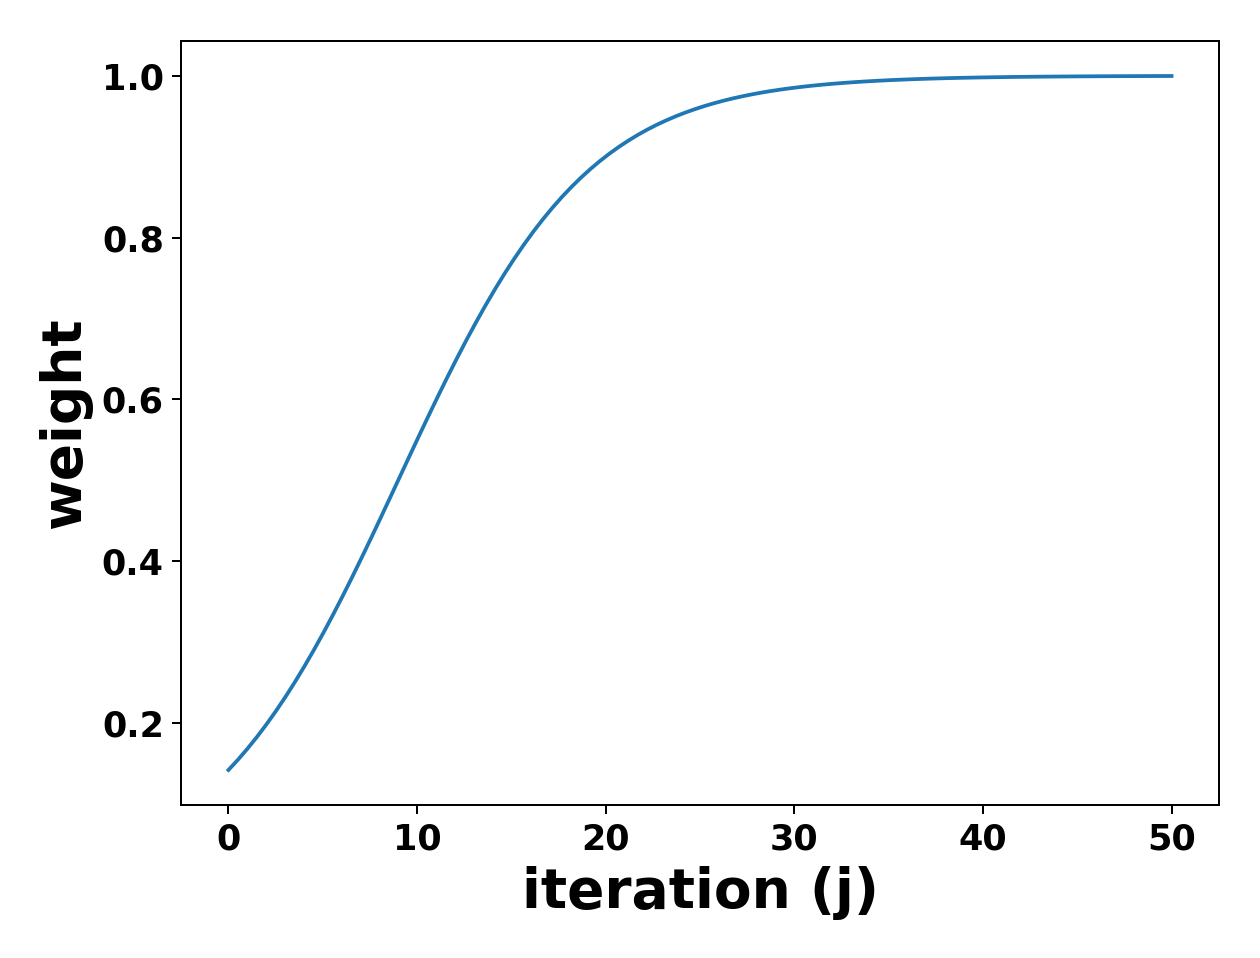
\includegraphics[width=0.45\linewidth]{figures/sigmoid.png}}%
\caption{(a) Histogram of sample durations (b) Sigmoid-like weight function used in single-time activation according to the Equation \eqref{eq:weight}.}f
\label{fig:sigmoid}
\end{figure}


\subsection{Single-time Activation}
\label{subsec:sta}
In real-time gesture recognition systems, it is extremely important to have smaller reaction time and single-time activation for each gesture. Gavrila et al.\cite{Gavrila1999TheVA} states that dynamic gestures have \textit{preparation}, \textit{nucleus} and \textit{retraction} parts. Out of all parts, nucleus is the most discriminative one, such that we can decide which gesture is performed even before it ends.  \\

Single-time activation is achieved through two level control mechanism. Either a gesture is detected when a confidence measure reaches a threshold level before gesture actually ends (early-detection), or the gesture is predicted when the detector deactivates the classifier (late-detection). In late-detection, we assume that the detector should not miss any gesture since we assured that detector has a very high recall rate. \\
\begin{figure}[t!]
	\centering
	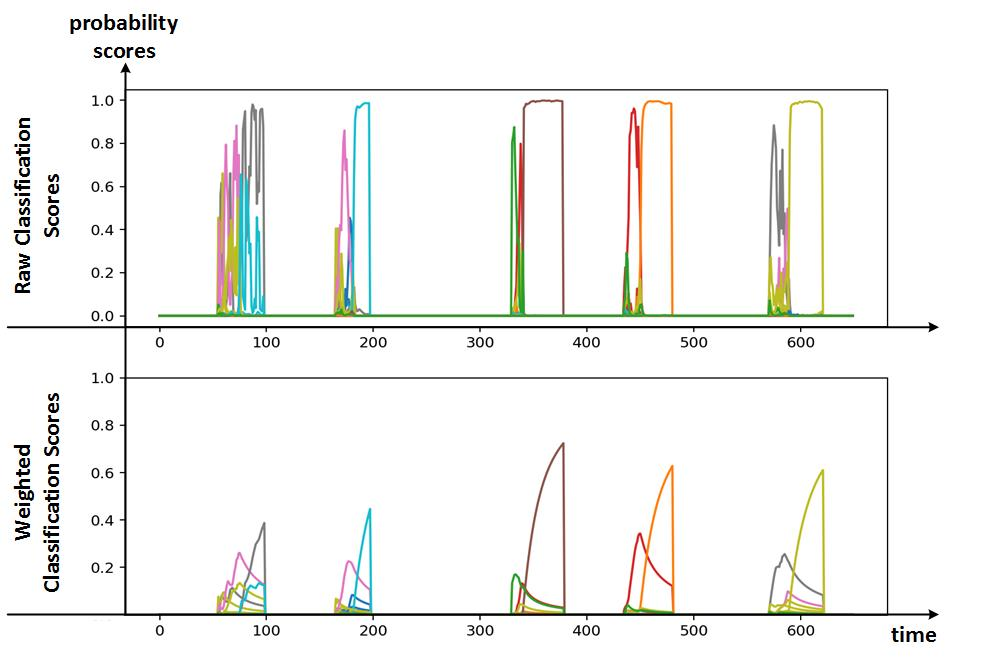
\includegraphics[width=\textwidth]{figures/weight_effect.jpg}
	\caption{Raw and weighted classification scores(top and bottom respectively). In top image we can see a lot of noise in the beginning of all gestures; however, near to the end of each gesture the classifier classify with more confidence. as The bottom image shows that we are able to cancel out this noise part through assigning smaller weights to the beginning part of gestures.}
	\label{fig:weight}
\end{figure}

The most critical part of the early-detection is that, the gestures should be detected after their nucleus parts for a better recognition performance. Because, several gestures can contain a similar preparation part which creates an ambiguity at the beginning of the gestures, as can be seen on the top graph of Figure \ref{fig:weight}. Therefore, we have applied weighted-averaging with a weight function as in Figure \ref{fig:sigmoid} (b), and its formula is given as,

\begin{equation}
    \label{eq:weight}
    w_j = \frac{1}{(1+\exp^{-0.2\times(j-t)})}
\end{equation}
    
\noindent where $j$ is the iteration index of an active state, at which a gesture is detected, and $t$ is selected as 9 by using the following formula,

\begin{equation}
    t = \frac{f}{2 \times s}
\end{equation}

\noindent where $f$ corresponds to the mean duration of the gestures(in number of frames) and $s$ is the stride length. This parameters allow us to have 0.5 and higher weights in nucleus part of the gestures on average. Figure \ref{fig:weight} shows the probability scores of five gestures over each iteration and their corresponding weighted-averages. It can easily be observed that we successfully cleared out the ambiguity of the classifier at the preparation part of the gestures.\\
\begin{algorithm}[t!]
	\renewcommand{\algorithmicrequire}{\textbf{Input:}}
	\renewcommand{\algorithmicensure}{\textbf{Output:}}
	\caption{Single-time activation in real-time gesture recognition }
    \centering
	\label{online_testing}
	\begin{algorithmic}[1]
		\Require Incoming frames from video data.
		\Ensure Predicted gestures.
		\For{each "frame-window" $w_i$ of length $m$}
		\If{a gesture is detected}
		\State{state $\leftarrow$ "Active"}
        \State {$\alpha \leftarrow probs_{j-1}\times(j-1) $}
        \State {$mean_{}probs = (\alpha + w_j\times probs_{j})/j$ }
        \State {$(max_1,max_2)=\max\limits_{gesture}{[mean_{}probs]_2}$ }
        \If{$(max1 - max2) \geq \tau_{\mathbf{early}}$}
        \State {\textit{early-detection} $\leftarrow$ "True"}
        \State \Return {gesture with $max_1$}
        \EndIf
        \State {$j \leftarrow j + 1$}
        \EndIf
        \If{the gesture ends}
        \State{state $\leftarrow$ "Passive"}
        \If{\textit{early-detection} $ \neq$ "True" \& $max_1 \geq \tau_{\mathbf{late}} $}
        \State \Return {gesture with $max_1$}
        \EndIf
        \EndIf
        \State {$i \leftarrow i + 1$}
        \EndFor
	\end{algorithmic}
\end{algorithm}

With this weighted-averaging strategy, we force our single-time activator to make decision at mid-late part of the gestures after capturing their nucleus parts. On the other hand, we need a confidence measure for early-detections in real-time since the duration of gestures varies. Hence, we decided to use the difference between weighted average scores of each classes as our confidence measure for early-detection. If detector switched on classifier, weighted average of probabilities for each class is calculated at each iteration. If the difference between two highest average probabilities is more than a threshold $\tau_{early}$, then early-detection is triggered; otherwise, we wait for the detector to switch off the classifier and the class with highest score above $\tau_{late}$ is predicted as late-detection. Details for this strategy can be found in Algorithm \ref{online_testing}. In our experiments we decided to fix $\tau_{late} = 0.15$ for simplicity. Also, its value is not so much important when the detector works well.\\

\section{Evaluation of Activations}
%As opposed to offline testing that uses standard metrics like accuracy,  recall, precision, etc...,  in online (real-time) testing evaluation of results is not only about how many of the gestures are correctly predicted but also many predictions.  Because of this reason, we used Levenshtein distance as our distance measure in online experiments evaluation. The Levenshtein distance is a sequence metric that measures the distance between sequences by counting the number of item-level changes (insertion,  deletion,  or substitutions) to transform one sequence into the other.  In our case, video sample and gestures in this video correspond to a sequence and items in this sequence, respectively.  For example, if our results for one video with gestures [1, 2, 3, 4, 5, 6, 7] are [0, 1, 2, 4, 5, 5, 6, 7], then the Levenshtein  distance  is 3 (deletion  of ”0”, substitution of ”5” to ”6” and  insertion  of ”3”).  In our metrics, we averaged this distance over the number of true target classes. For this case, the average distance  is $3/7 = 0.4285$, and we subtracted this value from 1 as we want to measure closeness (in this work it is referred as the Levenshtein  closeness) of our results,  which is equal to $(1-0.4285)/100 = 57.15\%$.\\
As opposed to offline testing which usually considers only about how many of the gestures are correctly predicted, we must also consider the following scenarios for our evaluation:

\begin{itemize}
    \item Misclassification of the gesture due to the classifier,
    \item Not detecting the gesture due to the detector,
    \item Multiple detections in a single gesture.
\end{itemize}


Considering these scenarios, we propose to use the Levenshtein distance as our distance measure in the evaluation of our online experiments. The Levenshtein distance is a sequence metric that measures distance between sequences by counting the number of item-level changes (insertion, deletion, or substitutions) to transform one sequence into the other. For our case, one video and gestures in this video  correspond to a sequence and items in this sequence, respectively. For example, lets consider the following ground truth and predicted gestures of a video:

\begin{align*}
    & Ground Truth\phantom{aa1}  [1, 2, 3, 4, 5, 6, 7, 8, 9]  &\\
    & Predicted\phantom{aaaa,}  [1, 2, 7, 4, 5, 6, 6, 7, 8, 9] &
\end{align*}

For this example, the Levenshtein distance is 2: The deletion of "6" which is detected two times, and the substitution of "7" to "3". We averaged this distance over the number of true target classes. For this case, average distance is $2/9 = 0.2222$ and we subtracted this value from 1 as we want to measure closeness (in this work it is referred as the Levenshtein metric) of our results, which is equal to $(1-0.2222)/100 = 77.78\%$ .\\

As we averaged the Levenshtein accuracy over true targets, it is possible that the accuracy became less than $0$. For such cases, we applied following equation: $\min(0,accuracy)$. \\

%Besides the Levenshtein metric, it is important to measure how precise (refered as "real-time precision") and sensitive (referred as "real-time recall") the predictions are. Real-time precision means the proportions of predicted classes that are in true classes in one sequence (video), and real-time recall means  the proportion of actual positives that are correctly identified in the same sequence. For the example given above, recall would be 100\% as all true gestures are included in the predicted ones, precision, on the other hand, would be $1-(1/8) = 87.5\%$ since 1 out of 8 predicted gestures (which is gesture "0") does not exist among true classes. \\